%Folgende Zeile aktivieren und als SVN property "svn:keywords" auf "Id" setzen, um SVN Versionsinformationen im Dokument zu erhalten
%\svnInfo $Id: einleitung.tex 60 2012-01-26 15:56:06Z koppor $ 

\chapter{Beschreibung der zu untersuchenden Daten}
Die Ergebnisse der Messungen werden in zwei verschiedenen Formaten untersucht:

\begin{enumerate}
\item \textbf{3D-Voxeldaten} \\
In ihrer ursprünglichen Form liegen die Daten in Form von dreidimensionalen Rastergrafiken, zusammengesetzt auf volumetrischen Pixel, vor. Diese Pixel werden üblicherweise als Voxel bezeichnet und sind Teil eines Voxelgitters. Jeder Voxel besitzt einen Wert, der seine Opazität wiedergibt. Der Wert dieser Opazität leitet sich direkt aus der beim CT gemessenen Dichte ab.

\begin{figure}[H]
  \begin{center}
    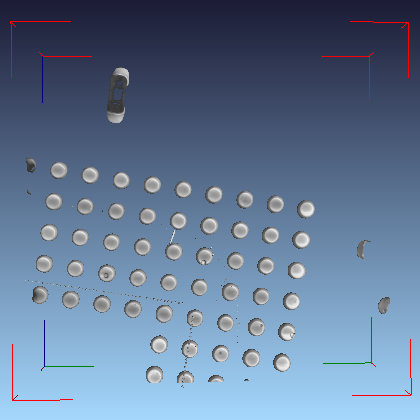
\includegraphics[width=0.5\textwidth]{3ddata.png}
    \caption{3D-Voxeldatensatz in myVGL}
    \label{fig:3ddata1}
  \end{center}
\end{figure}

\item \textbf{2D-Slices} \\
Die zweidimensionalen Slices werden auf Basis der 3D-Voxeldaten berechnet. Dabei wird eine Schicht des Voxelgitters extrahiert und auf Basis der Opazitätswerte eine Rastergrafik erstellt, wobei jeder Pixel eindeutig einem Voxel zugeordnet werden kann. Durch diese Umformung können bei der Objekterkennung auch 2D-Verfahren genutzt werden.

\begin{figure}[H]
  \begin{center}
    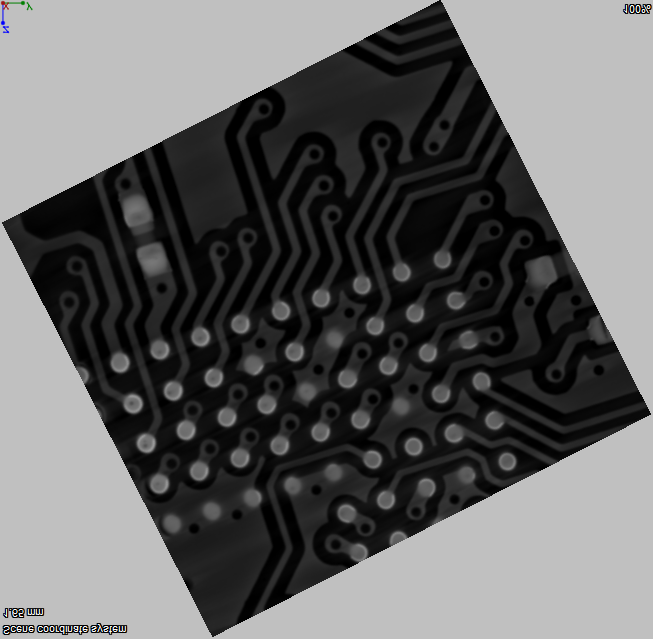
\includegraphics[width=0.5\textwidth]{2ddata.png}
    \caption{2D-Voxeldatensatz}
    \label{fig:3ddata1}
  \end{center}
\end{figure}

\end{enumerate}
